\documentclass{IET}

\usepackage[utf8]{inputenc}
\usepackage[english]{babel}
\usepackage{amsmath}
\usepackage{amsfonts}
\usepackage{amssymb}
\usepackage{graphicx}

\begin{document}

\title{A CNN-based Cow Interaction Watchdog}
\author[1*]{Håkan Ardö}
\affil{Centre for Mathematical Sciences, Lund University, Sölvegatan 18, Lund, Sweden}
\author[2]{Oleksiy Guzhva}
\affil{Swedish University of Agricultural Sciences, Department of Biosystems and Technology, Växtskyddsvägen 3, Box 103, 23053 Alnarp, Sweden}
\author[1]{Mikael Nilsson}
\author[2]{Anders Henrik Herlin}
\affil[*]{ardo@maths.lth.se}

\abstract{
Animal behaviour and welfare can be studied and assessed by looking at different interactions occurring between the animals. Video recordings of a scene of interest are often made and then watched/evaluated by experts. However, the  interactions of interest are often fairly rare. To reduce the amount of time the experts spend on watching the uninteresting video, this paper introduces an automated watchdog system that can discard some of the recorded video material. A pilot study on cows was made where a Convolutional Neural Network (CNN) detector was used to count the number of cows in the scene and discard video where less than two cows were present. This removed 38 \% of the recordings while only losing 1 \% of the interesting video. If also the distance between the cows present in the scene was considered, then 50 \% of the recordings could be remoed without loosing more than 4 \% of the interesting frames.
}

\maketitle

\section{Introduction}

Scientists working with animal behaviour and welfare are interested in studying the social interactions between cows in dairy farms. Typically these studies are performed by defining a set of interactions such as head butting, body pushing, social licking, and other physical and non-physical contacts. Every interaction is described in detail in a protocol. Then an expert studies the area of interest for a considerable amount of time and counts the number of each interaction occurring or the duration of the interaction. This is performed for the whole duration of the video sequence/sequences used for the particular study \cite{MartinandBateson2007}. Some of these interactions are relatively rare, which means that much expert time has to be spent in looking at raw video data to find potentially interesting sequences.

Some recent studies on cow behaviour in the dairy barn environment were based on different GPS or wireless sensor network (WSN) solutions \cite{Nadimietal2012}. These solutions allow scientists to see spatial distribution of animals and to measure varying levels of activity \cite{Nadimietal2012}. However, the number and complexity of behaviours that could be monitored with the position-based approach is limited. Therefore, new methods based on video surveillance and image analysis, which could extend the number of parameters for studying, are of great importance. Correct classification of interaction is of importance as some interactions are positive, friendly and strengthens the bond between animals and others are possibly deleterious and can reflect a struggle for resources.

In this paper, the objective was to take the first step towards an automated system for behavioural analysis. The study area was filmed using video cameras. Then an automated watchdog system will remove unnecessary parts (e.g. those, containing events that are not relevant or without animals in the scene) of the recorded video material. The remaining video sequences will still have to be studied by experts, but the time spent looking at uninteresting video sequences will be significantly reduced. 

This is achieved by developing a cow detector that detects cows in the scene and represents them with rotated bounding boxes. That means the number of cows can be counted and distances between the cows can be measured. Rotated bounding boxes allow much more precise distance measures between diagonally oriented cows as compared to more classical non-rotated bounding boxes due to the elongated aspect ratio of the cows.

The pilot study used to develop this watchdog was made in a dairy barn in the south of Sweden with 252 Swedish Holstein cows. Cows were milked by four automatic milking robots, which had a common waiting area (6x18 meters). This waiting area is a common space which cows that are ready for milking are allowed to enter at any point in time. They may then interact with each other in order to decide the order of entry to each of the milking robots. A direct relationship between cows' inter-cow distance and their aggressive behavioural patterns was demonstrated by \cite{DeVriesetal2004}. Other studies \cite{Hemsworth2003, Kilgour2012} showed certain effects of inferior animal welfare connected to the restrained performance of their natural behaviour. Therefore, early diagnostics of unconditional changes in animal behaviour when linked to health and welfare could not only save time and money for the farmer but also decrease the production pressure for every animal in the barn \cite{Polikarpusetal2015}.

\subsection{Related work}
Most previous work on detecting cows by using video cameras have been focused on monitoring areas where the orientation of the cows was known due to physical limitations imposed by the surroundings. Two examples of this are the Viola-Jones based detector of Arcidiacono et al. \cite{Arcidiacono2012} for detecting cows at the feed barrier and the work of Martinez-Ortiz1 et al. \cite{martinez2013video} to detect and track cow heads in narrow entrance corridors. There are also approaches that rely on more advanced sensors, such as Abdul et. al \cite{abdul2016locomotion} that uses a depth camera.

The current state of the art for detecting cows freely moving around was presented by Porto et al. \cite{porto2015automatic}. They use a Viola-Jones based detector and need 
6 cameras at 4.6 meters height to cover a $15.4 \times 3.8$ m area and detects cows in 3 different orientations: vertical, horizontal and diagonal with a hit rate of 90\%. They do not use separate detectors for the two different diagonals which mean that producing rotated bounding box from their results would not be straight forward. In the work presented in this paper, only 3 cameras at 3.6 meters height were needed to cover a $18 \times 6$ m area and detect cows in 32 different orientations with a hit rate of 97\%. Note that the hit rates are from different datasets, and that the dataset used in this article have larger variations in viewpoints due to the use of fewer cameras at a lower height to cover a larger area.

General purpose object detection frameworks such as YOLO \cite{DBLP:journals/corr/RedmonDGF15,redmon2016yolo9000} and SSD \cite{liu2016ssd} have very good performance. They do however focus on detecting objects of varying size and aspect ratio but with fix orientation. In the scenario considered in this paper, the size and aspect ratio is fixed and known while orientation (rotation) varies and have to be estimated. 

He et al. \cite{He_2015_ICCV} have considered rotated bounding boxes to generate general purpose objected proposals. They do a local optimization over position, size, aspect ratio and rotation from an initial set of sampled widows. In the proposed approach the size and aspect ratio are known and fixed and an exhaustive search over position and rotation is performed. That way there the risk of not considering relevant rotations is eliminated. Also, He et al. \cite{He_2015_ICCV}  is based on hand crafted features assuming that image borders are unlikely to contain objects, and that the object of interest covers a significant part of the interior of the image.

Another approach is to combine segmentation algorithms such as
DeepMask \cite{DBLP:journals/corr/PinheiroCD15} and
SharpMask \cite{DBLP:journals/corr/PinheiroLCD16} with an object detector shuch as 
MultiPathNet \cite{DBLP:journals/corr/ZagoruykoLLPGCD16}. This results in object detections augmented with pixel level segmentations. From those segmentations rotated bounding boxes could be generated or, even better, distance measures can be made using the segmentations directly. However this approach requires manual pixel level segmentations as training data while the suggested approach only requires a few manual clicks per training object.

\subsection{Experimental setup}

\begin{figure}[tb]
\begin{center}
  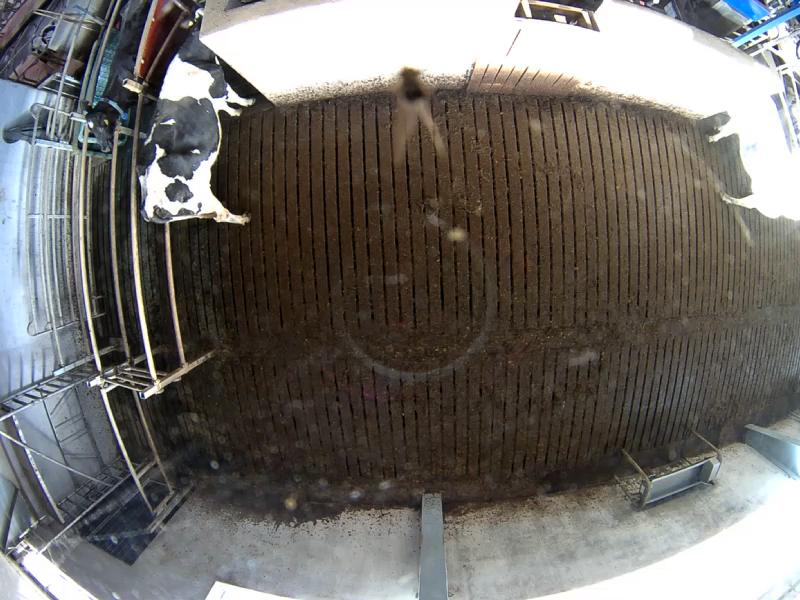
\includegraphics[width=0.3\textwidth]{old-2.jpg}
  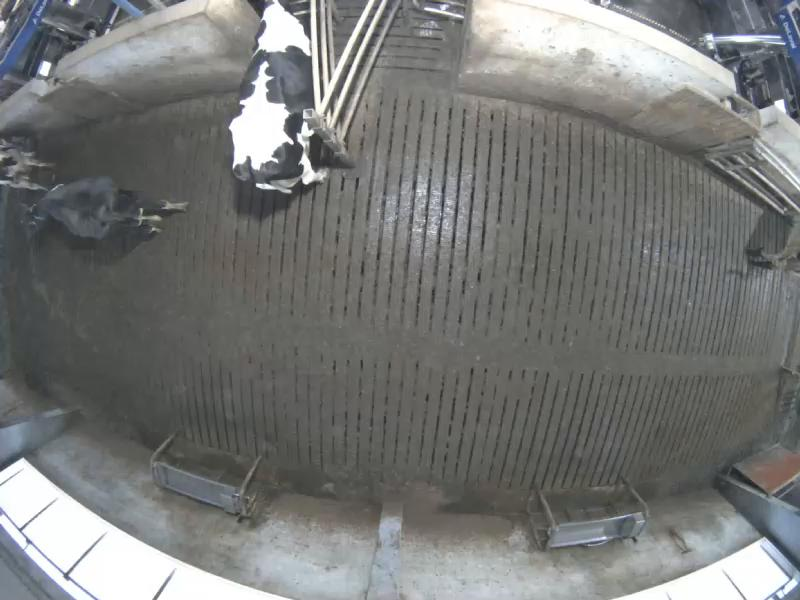
\includegraphics[width=0.3\textwidth]{old-1.jpg}
  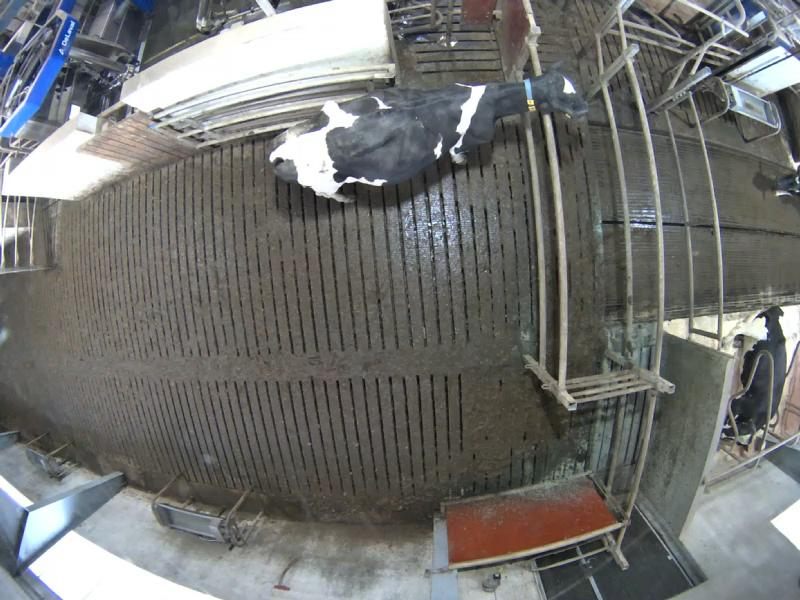
\includegraphics[width=0.3\textwidth]{old-0.jpg}
\end{center}
  \caption{Example frames the recorded video.}
  \label{fig:old}
\end{figure}


Video recordings were made using three Axis M3006-V cameras with a wide field of view, 134 degrees. They were placed in the ceiling at an height of 3.6-meters, pointing straight down to optimise overview over the study area. There was a significant overlap between the camera images to not miss events taking place at the border between the cameras. See Figure~\ref{fig:old} for some example frames. In total 2315 hours (1 month) of 800x600 video at 16 Frames Per Second (FPS), was collected.

The cameras were calibrated to compensate for lens distortion and rectified. Although the cameras were physically mounted to point fairly straight down, they were still slightly tilted. This tilting was synthetically removed during the rectification. The result of this calibration is video images where the cows have the same size regardless of where in the image they appear. Also, the scan-lines of the three different cameras become aligned, which allows them to be stitched together to form an overview of the entire waiting area.

Finally, a Convolutional Neural Network (CNN)  was trained to detect the cows in the images, and statistics about how many cows and their distances/relation to each other was extracted. Using that statistical data, scientists working in a field of animal behaviour could form queries to select particular time intervals to watch, such as "show me video clips involving at least two cows with the neck of one cow closer than one meter to the body of the other".


\section{Camera calibration}

\begin{figure}[t]
\begin{center}
  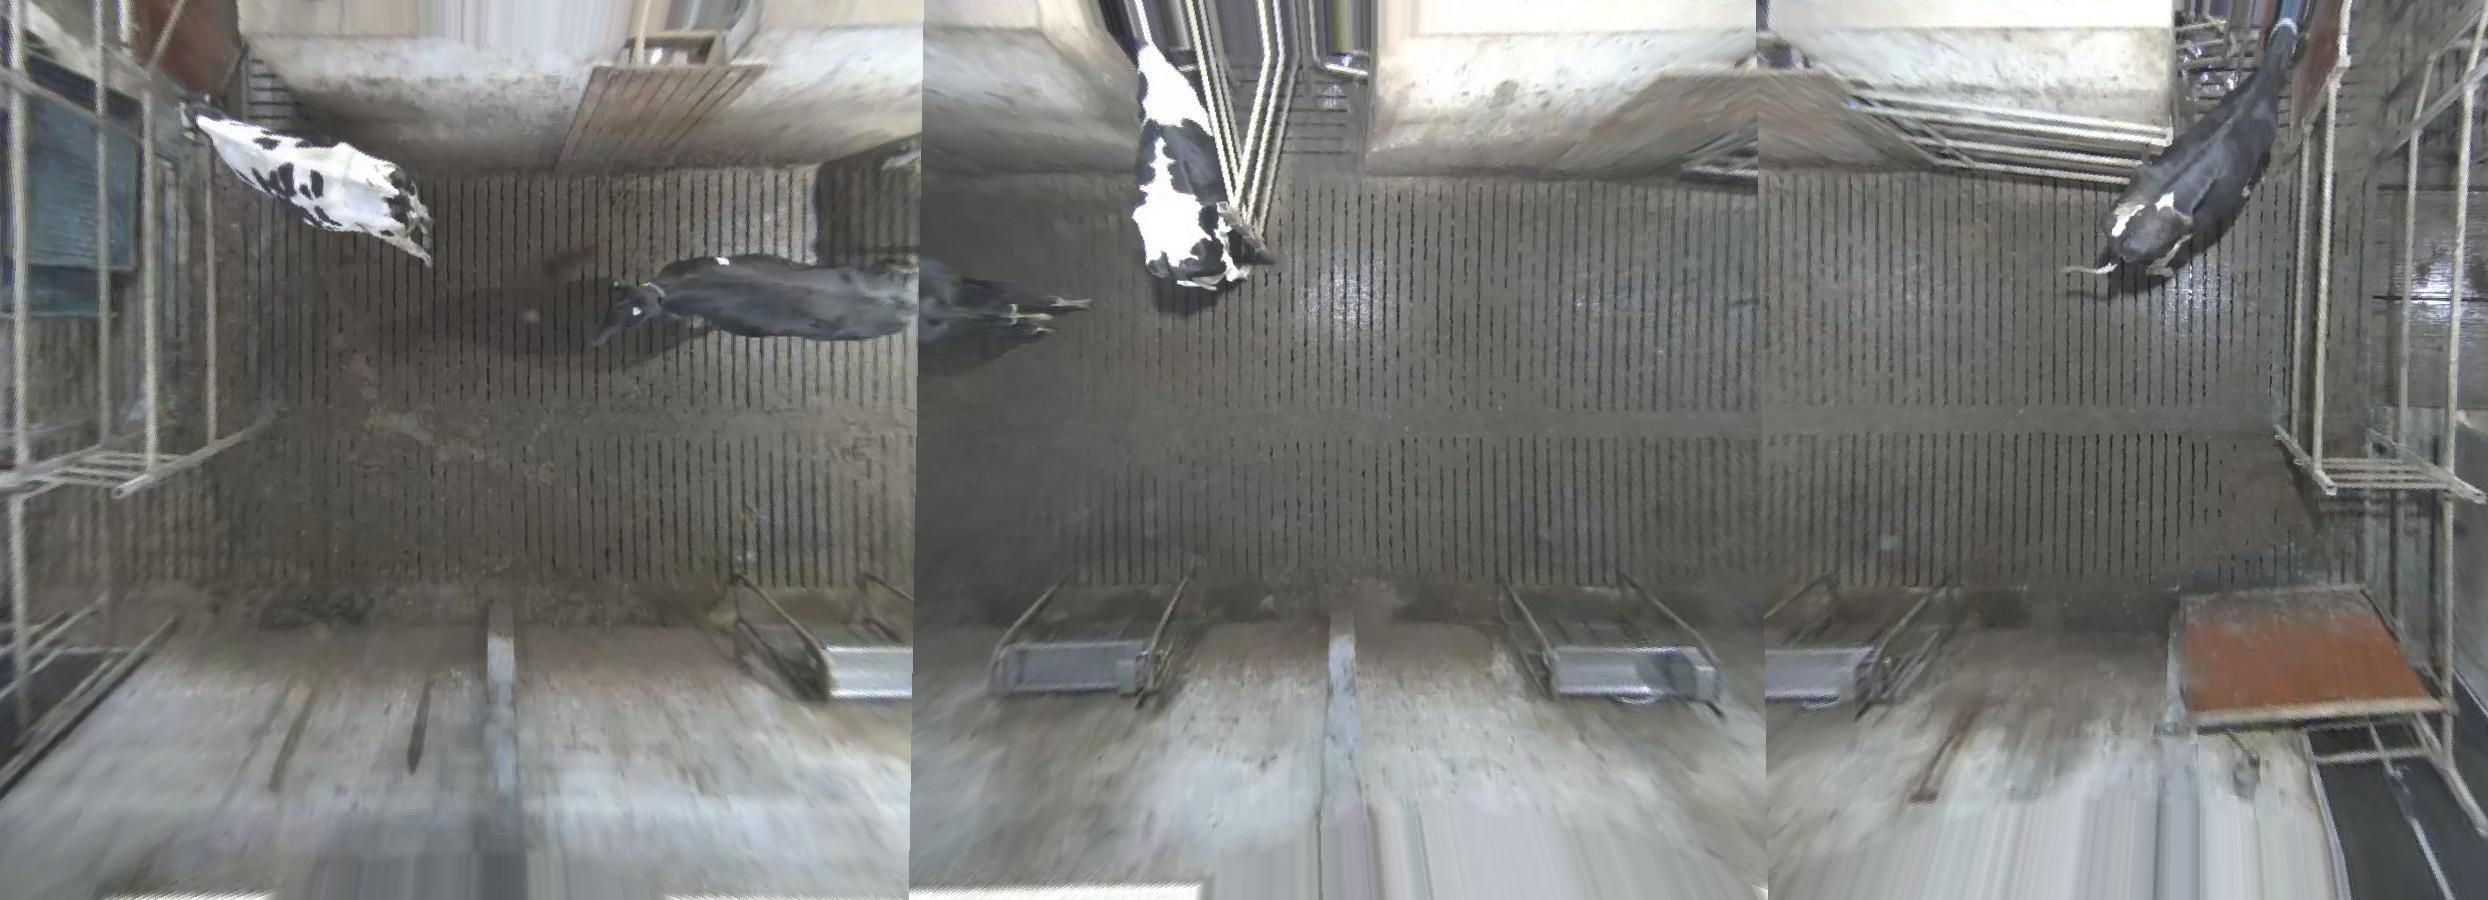
\includegraphics[width=0.9\textwidth]{full.jpg}
\end{center}
  \caption{The frames from Figure~\ref{fig:old} projected onto the cow shoulder plane and stitched together}
  \label{fig:stitch}
\end{figure}

\begin{figure}[b]
\begin{center}
  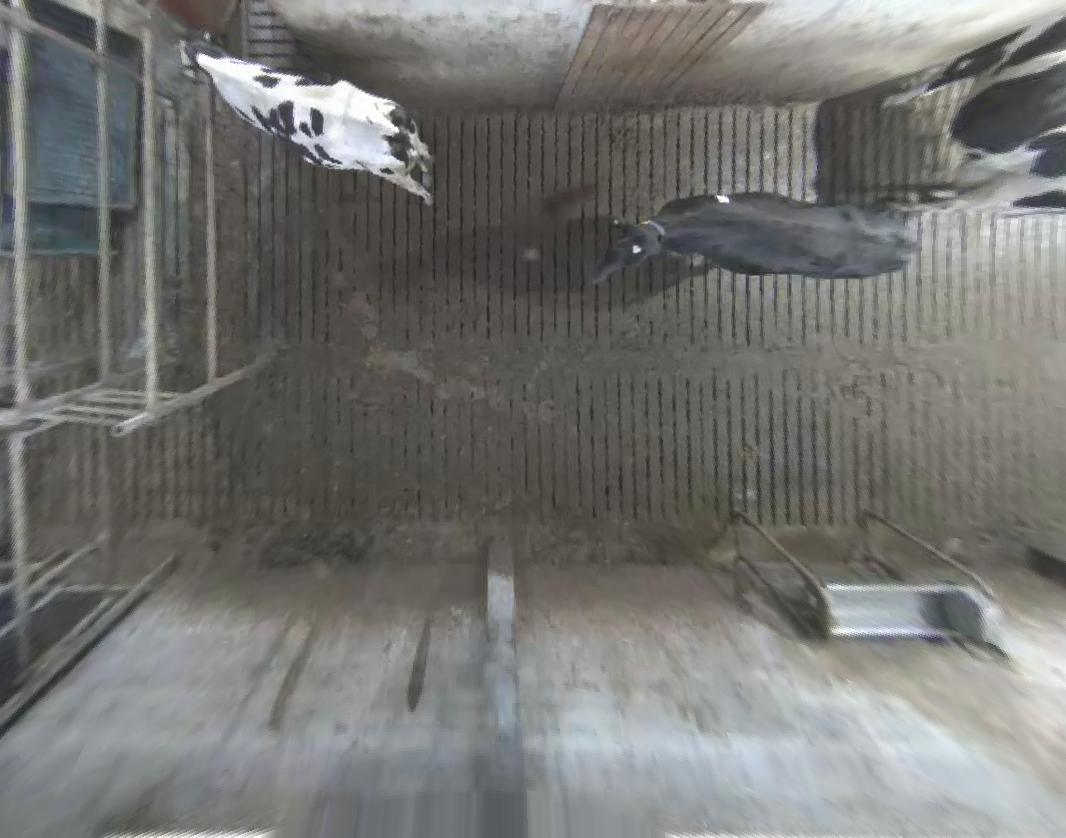
\includegraphics[height=0.15\textheight]{left_single.jpg}
  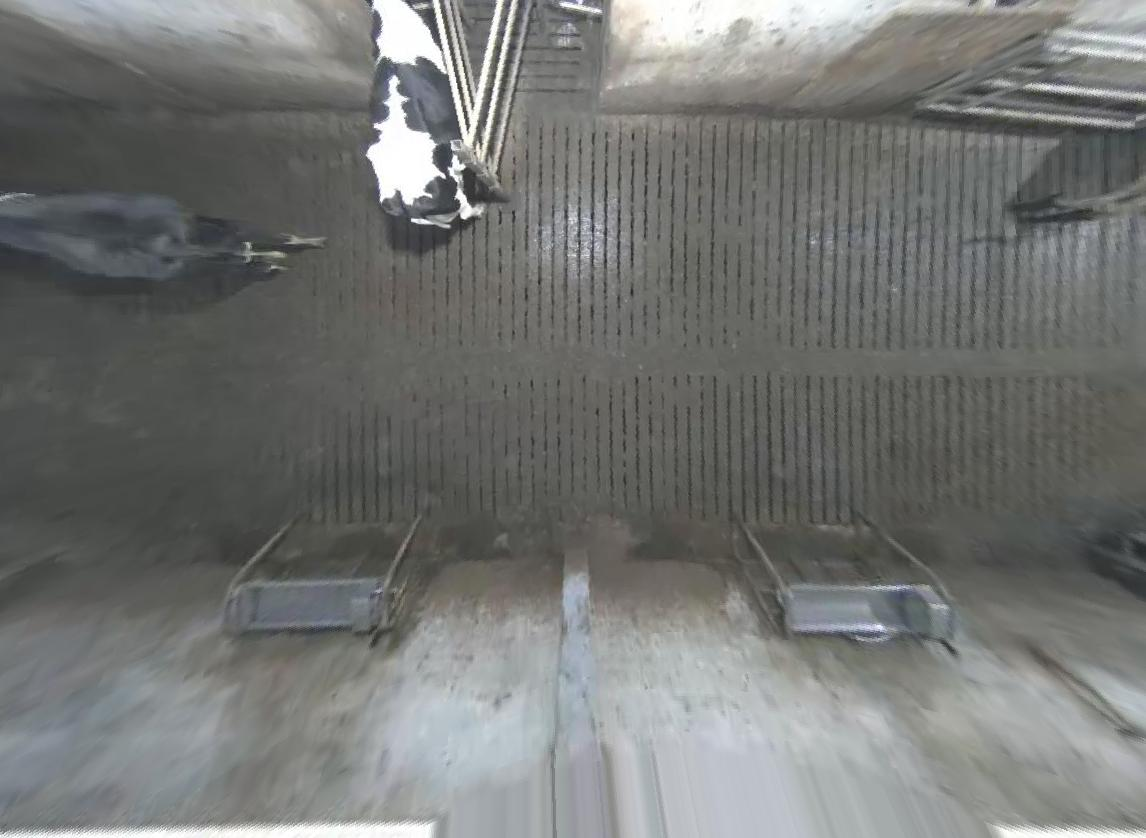
\includegraphics[height=0.15\textheight]{mid_single.jpg}
  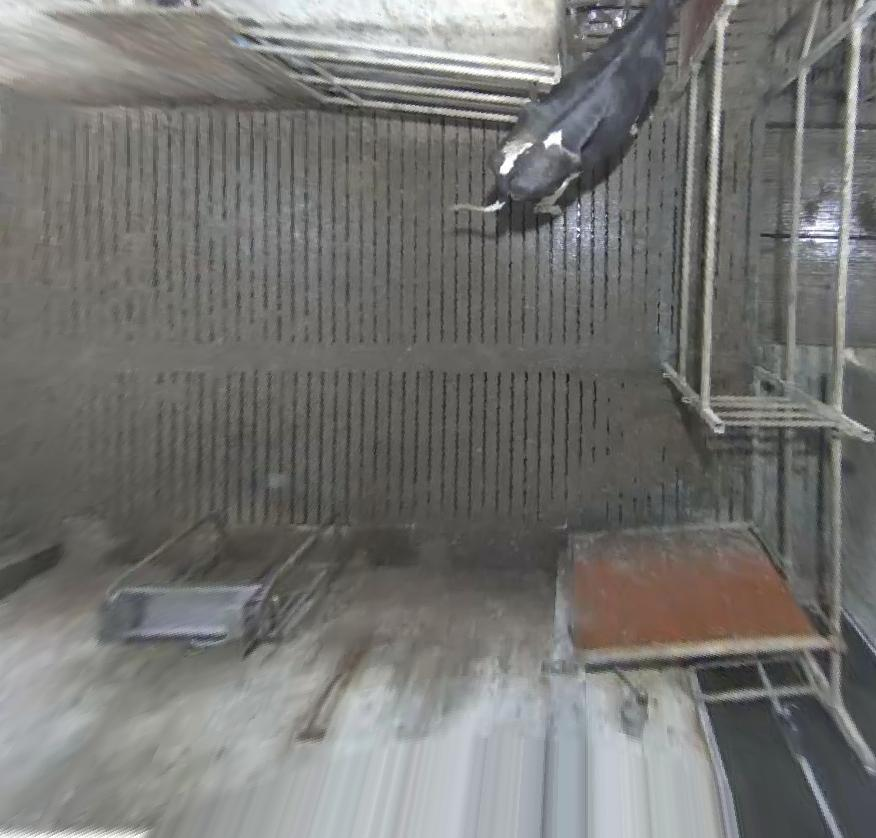
\includegraphics[height=0.15\textheight]{right_single.jpg}
\end{center}
  \caption{Dewarped frames from each of the cameras with overlaps to allow the detector to process them one by one.}
  \label{fig:separate}
\end{figure}



The classical pinhole camera model augmented with a lens distortion model was used to model the camera.
The camera setup was calibrated by placing markers on the walls and stands in the middle of the room. They were all placed at the same height and thus defined a plane. The mean cow height in the barn was measured, and the plane was placed at their shoulder height. This height was estimated to be 1.49 meters with a standard deviation of 0.05 by measuring twelve random cows in the study area.
This is the plane in which all of the landmarks considered below, except for the head, are expected to be found. By projecting detected landmarks back and forth between the camera images and this plane, detections from different cameras can be matched.

In addition to the markers, the focal length and lens distortion parameters were provided by the camera manufacturer.
The lens distortion was removed, and a homograph was estimated that projected each of the camera images onto the cow shoulder plane. Figure~\ref{fig:stitch} shows a view stitched together from all three images in Figure~\ref{fig:old}. It shows an overview of the entire waiting area. At the borders between the cameras, the image becomes strange as cows there are viewed from different directions on opposite sides of the border. However, this image is only used for illustration. There is enough overlap between the images to allow them to be processed one by one and then the resulting detections can be combined using this calibration. Figure~\ref{fig:separate} shows the separate dewarped frames used by the detector. Note how the same cow is almost fully visible in both the left and the middle image.

By using homogeneous coordinates, the pinhole camera model that forms 2D image pixels, $x=\left(x_1, x_2, 1\right)$, by projecting world 3D points, $X=\left(X_1, X_2, X_3, 1\right)$, using a camera matrix, $P$, can be formed as

\begin{equation}
	\lambda x = P X = K \left(
	\begin{array}{cc}
		R & t \\
	\end{array}
	\right) X = 
	\left(
	\begin{array}{ccc}
		f & 0 & p_x  \\
		0 & f & p_y  \\
		0 & 0 & 1  \\
	\end{array}
	\right)
	\left(
	\begin{array}{cc}
		R & t \\
	\end{array}
	\right) X,	
\end{equation} 
were $f$ is the focal length of the camera and $\left(p_x, p_y\right)$ its principal point while $t$ and $R$  define its 3D position and orientation. This projective image is then distorted using some lens distortion function, $\hat x = f_\text{dist}\left(K^{-1}x\right)$. Here a radial fish eye lens distortion model is used. By using nominal image coordinates, $\lambda x_n = K^{-1} x$ and $\hat x_n = \left(\hat x_1 - p_x, \hat x_2 - p_y, 1\right)$ the inverse of this distortion function can be express as 

\begin{equation}
	\left| x_n \right| = \tan \left( \sum_i k_i \left| \hat x_n \right|^i \right)
	\label{eq:dist} ,
\end{equation}
where $k_i$ is the set of distortion parameters and 
$\left| x \right| = \sqrt{x_1^2 + x_2^2}$.
Note that with this distortion model, the focal length becomes part of the distortion and Equation~\ref{eq:dist} allows the pixels produced by the camera $x$ to be transformed into nominal projective coordinates, $x_n$, directly. The distortion parameters, $k_i$, was provided by the manufacturer and the principal point, $\left(p_x, p_y\right)$,  was assumed to be at the center of the image.

In the camera images, the markers placed in the cow shoulder plane was located manually and their nominal coordinates, $x_n$, were registered by clicking on them. Also, real world distances between the marks were estimated using a laser pointer. From these measurements the world coordinates, $x_s$, were calculated using multidimensional scaling \cite{Young1938}. One homograph, $H$, for each camera was fitted to the point correspondences allowing the pixels to be projected onto this plane using 
\begin{equation}
\lambda x_d = H x_n .
\end{equation}

This generates a common coordinate system for all of the cameras which allows detections from each of the cameras to be projected into this common frame. That way different cameras could be used in different parts of the waiting area. To minimise the amount of occlusion taking place, each part of the waiting area should use the closest camera to get a view from as straight above as possible. For that, the camera position in the cow shoulder plane needs to be estimated. That can be achieved by RQ factorisation of $H$ \cite{Hartley2004}, 

\begin{equation}
H = K_d R_d = 
    \lambda
	\left(
	\begin{array}{ccc}
		f_x & s & c_x  \\
		0 & f_y & c_y  \\
		0 & 0 & 1  \\
	\end{array}
	\right)
	R_d ,
\end{equation}
were the camera position is given by $c = \left(c_x, c_y, 1\right)$. Figure~\ref{fig:stitch} shows an image where each pixel has been chosen from the camera closest to that pixel, i.e. with  minimum $\left| x_d - c \right|$. The final crops used from each camera consists of the pixels in this stitched view with a border of $75$ pixels added on each side to make the overlap $150$ pixels, which roughly corresponds to the length of one cow.


\section{Data annotation}

The complete dataset contains three months of recordings collected from 3 cameras at 16 fps. That makes 400 million frames. Among these 1722 was randomly selected and annotated. The annotation process started before everything was recorded, so the video is sampled somewhat more densely in the beginning but the mean distance between two adjacent annotated frames is 30 min. So we believe that the annotated frames are fairly uncorrelated and should give a good representation of the distribution of frames that could be expected to be seen from these cameras.

The annotated subset contained in total 6399 cows in the images. Each cow was annotated with seven landmark points: head, left and right shoulder, front middle, left and right hip and back middle. In addition to that one additional landmark "cow centre" was defined as the mean of front middle and back middle. This data was then used to train a CNN detector.


\section{CNN cow detector}

The detector was split into two steps. The first step is a fully convolutional CNN that detects the landmarks in the image. Currently, only four of the landmarks were used to speed up the experiments, but extending to use all seven is straightforward. The architecture of this network is a fully convolutional version of VGG \cite{Simonyan14c} with batch normalisation \cite{DBLP:journals/corr/IoffeS15} after each convolution step. Details are shown in Table \ref{tab:cownet}.

The second step is another CNN that works with the probability map produced by the first as input and tries to detect the cows and their orientations. The full circle is divided into 32 equally spaced orientations which generate 32 different oriented cow classes. In addition to that, there is the no cow class, which makes the total number of classes of this CNN 33. The input probabilities were turned into log likelihoods as it makes more sense when summing them together. Then the network consists of a single $ 13 \times 13 $ convolutional layer. Details are shown in Table \ref{tab:cowdirnet}.

\begin{table}
\begin{center}
\begin{tabular}{|l|c|c|}
\hline
\textbf{Layer type} & \textbf{Size} & \textbf{Channels} \\
\hline

Conv + BNorm + Relu & 3x3 & 32 \\
MaxPool(stride=2) & 2x2 &  \\
\hline

Conv + BNorm + Relu & 3x3 & 64 \\
MaxPool(stride=2) & 2x2 &  \\
\hline

Conv + BNorm + Relu & 3x3 & 128 \\
Conv + BNorm + Relu & 3x3 & 128 \\
MaxPool(stride=2) & 2x2 &  \\
\hline

Conv + BNorm + Relu & 3x3 & 256 \\
Conv + BNorm + Relu & 3x3 & 256 \\
MaxPool(stride=2) & 2x2 &  \\
\hline

Conv + BNorm + Relu & 3x3 & 512 \\
Conv + BNorm + Relu & 3x3 & 512 \\
MaxPool(stride=2) & 2x2 &  \\
\hline

Conv + BNorm + Relu & 1x1 & 1024 \\
Conv + BNorm + Relu & 1x1 & 1024 \\
Conv + Softmax & 1x1 & 5 \\
\hline

\end{tabular}
\end{center}
\caption{CNN architecture for landmark detection. 
%The input is an image of any size with 3 rgb channels scaled to the range $\left[0,\,1\right]$. The output is probability map segmenting the entire image into 5 classes: Ground, Cow front middle, Cow center, Cow back middle and Cow head.
}
\label{tab:cownet}
\end{table}

The landmark net was trained on patches of $150\times 150$ pixels extracted from the input images. This makes the output during training a single pixel. The positive examples were centred on the landmarks and randomly jittered $\pm 16$ pixels (as the distance between output pixels is $32$ input pixels). Negative patches were selected at centres more than $32$ pixels from any landmark. In addition to the positive and negative patches a set of do not care patches were selected at random centres at distances between $16$ and $32$ pixels from landmarks. The ground truth probability of these patches belong to the class of the landmark was set to $0.5$, and the probability that they are ground was set to $0.5$. In some cases, several landmarks appear within $32$ pixels of the patch centre. In that case, the probability mass was distributed uniformly among all involved classes.

The weights of the convolutions were initiated using random samples draw from a Gaussian
distribution truncated at $2\sigma$, with standard deviation $\sigma=\sqrt{\frac{2}{n}}$,
where $n$ is the number of inputs\cite{DBLP:journals/corr/HeZR015}. The networks were regularised with weight decay of
$0.0001$ and optimised using stochastic gradient descent with $0.9$ momentum. The
learning rate was initiated to $1.0$ and reduced by a factor $10$ each time the validation
error flattens. The landmark CNN uses only valid outputs from the convolutional and maxpool
layers while the cow detector keeps the same resolution also to detect cows that are
slightly outside the image.

\begin{table}
\begin{center}
\begin{tabular}{|l|c|c|}
\hline
\textbf{Layer type} & \textbf{Size} & \textbf{Channels} \\
\hline

MaxPool(stride=1) & 3x3 &  \\
Log & & \\
Conv + BNorm + Relu & 13x13 & 33 \\
Softmax & & \\
\hline
\end{tabular}
\end{center}
\caption{CNN architecture to detect oriented cows
%cows and their orientation. The input is the 5 channel probability map from the landmark detector with the last MaxPool removed to increase resolution. The output is a probability map that segments the image into either background or cow in one of 32 different orientations.
}
\label{tab:cowdirnet}
\end{table}

\begin{figure}[tb]
\begin{center}
  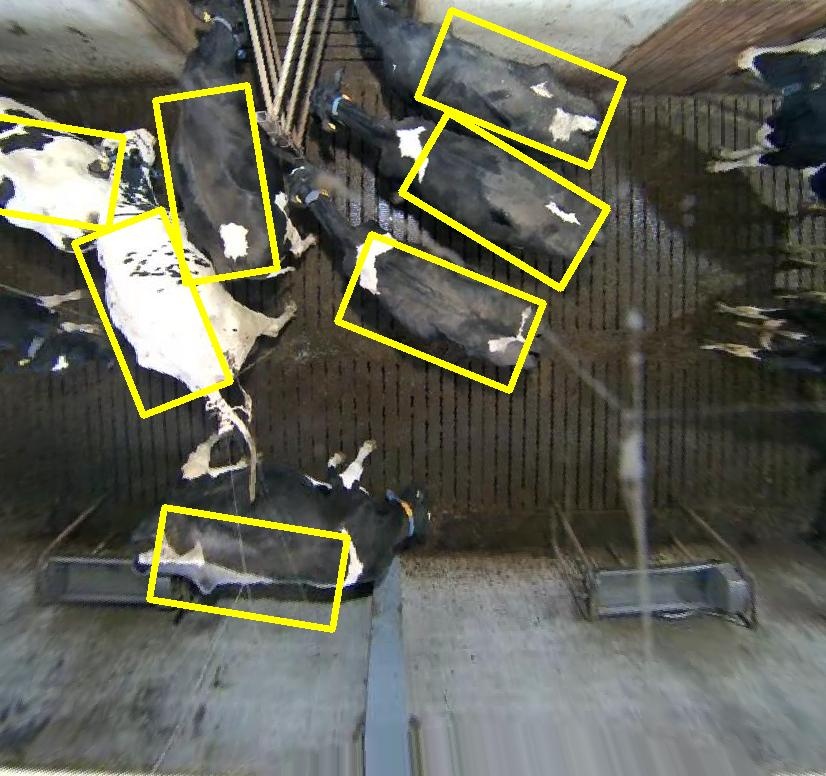
\includegraphics[width=0.25\textwidth]{ok/1419422172315416.jpg}
  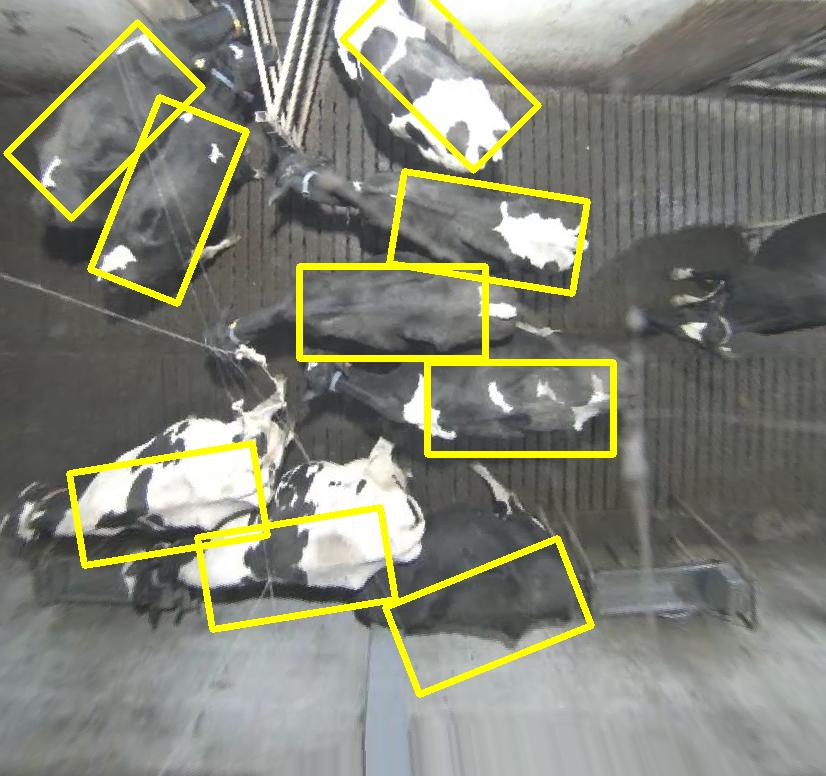
\includegraphics[width=0.25\textwidth]{ok/1419630968631761.jpg}
  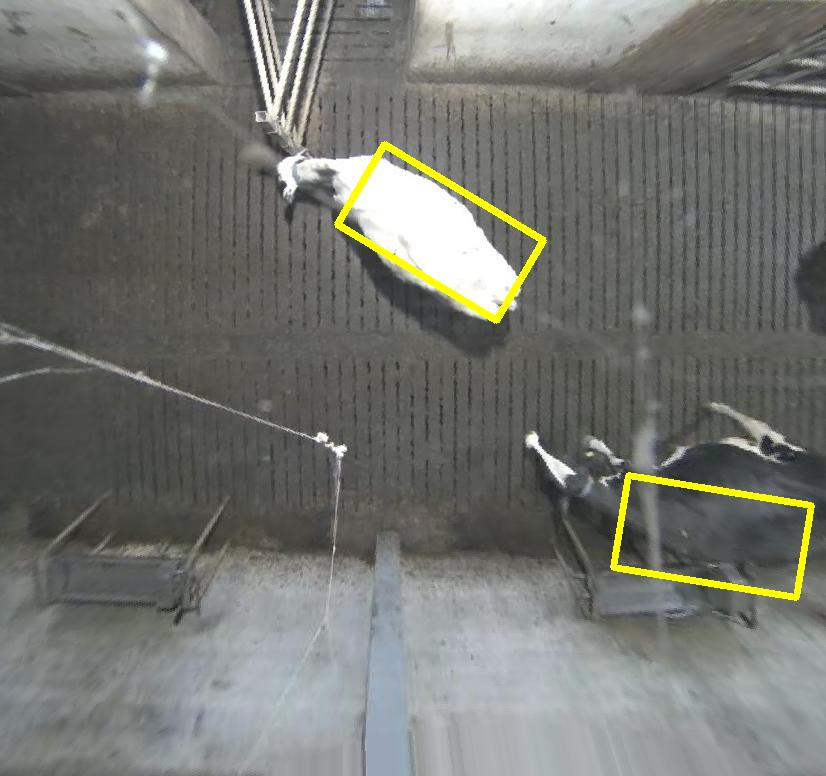
\includegraphics[width=0.25\textwidth]{ok/1420251135794580.jpg}

  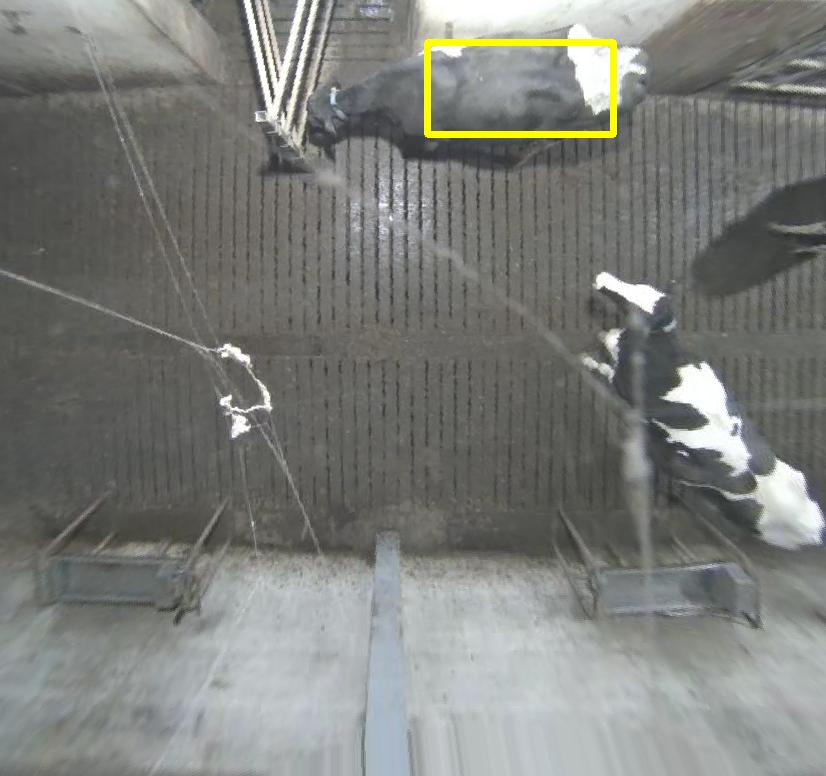
\includegraphics[width=0.25\textwidth]{bad/1419743355933936.jpg}
  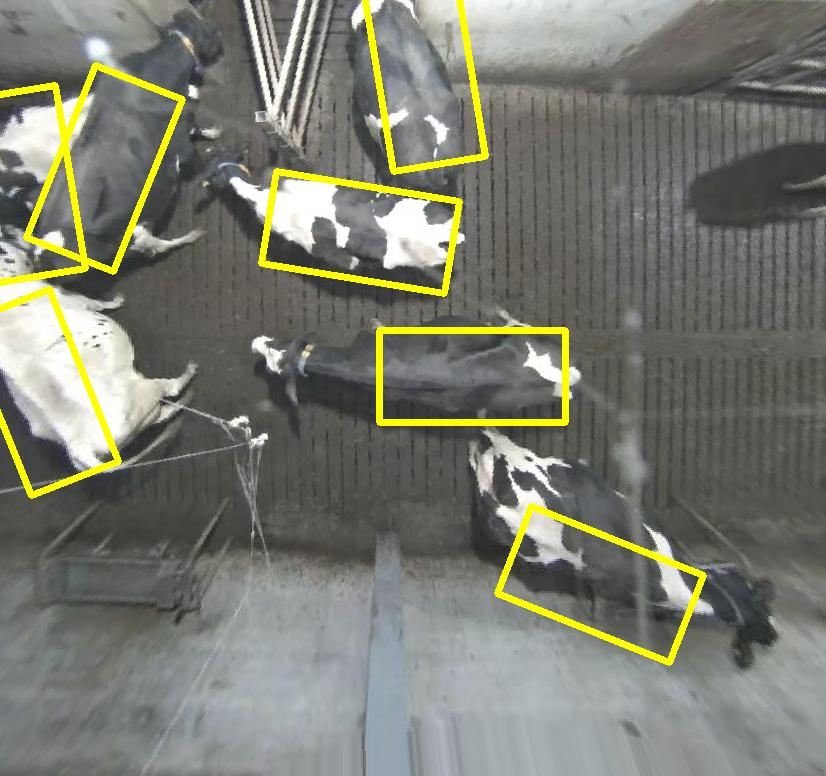
\includegraphics[width=0.25\textwidth]{bad/1420050868326145.jpg}
  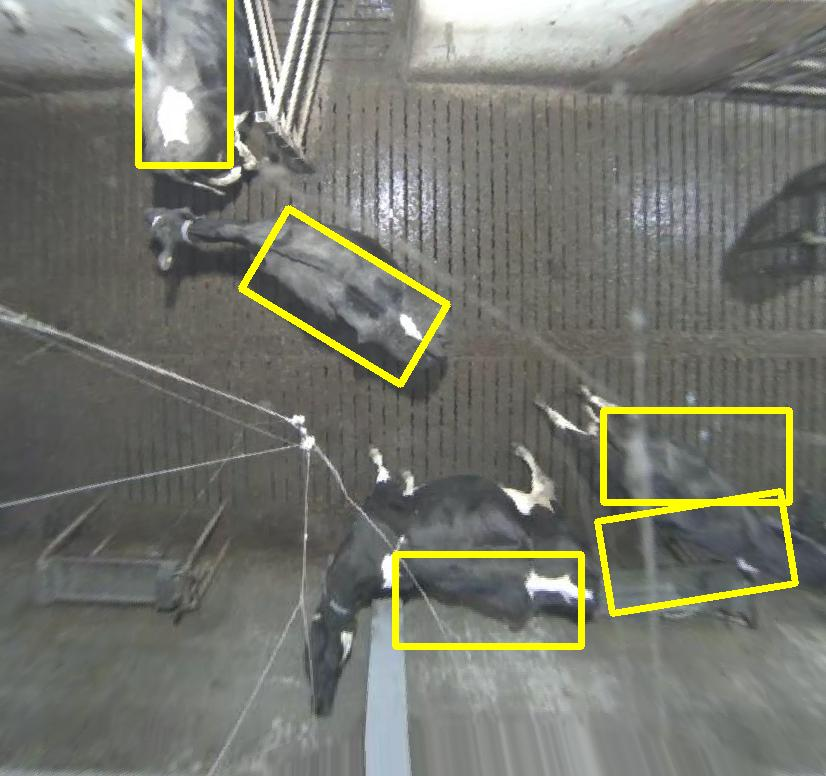
\includegraphics[width=0.25\textwidth]{bad/1420185482574217.jpg}
\end{center}
  \caption{Top row: Three images correctly interpreted (all cows detected and no extra detections). Bottom row: The three images were the errors were made (1 missed cow and two extra detections).}
  \label{fig:res}
\end{figure}

Once the net was trained, the step length of the last maxpool layer was reduced from two to one to increase the output resolution. The net was then applied to the full rectified training images producing probability maps of $44\times 46\times 5$ pixels. These were used as training examples for the cow detection net (without splitting them into patches). Output ground truth probability maps of $44\times 46\times 33$ pixels were constructed from the annotations by projecting each cow, $i$, center point into the probability map as $\left( x_i, y_i \right)$ and calculate its angle $a_i$ as the angle of the line between front middle and back middle landmarks. Then a binary $44\times 46\times 33$ mask $B\left( x, y, c \right)$ is formed, containing a background mask
\begin{equation}
B\left( x, y, 32 \right) = \left\lbrace
\begin{array}{clc}
0 & \text{if} &
\begin{array}{c}
 \lfloor x_i \rfloor \leq x \leq \lceil x_i \rceil \\
 \lfloor y_i \rfloor \leq y \leq \lceil y_i \rceil
\end{array}
\\
1 & \multicolumn{2}{l}{\text{otherwise}}
\end{array}
\right.
\end{equation}
and $32$ orientation masks
\begin{equation}
B\left( x, y, c \right) = \left\lbrace
\begin{array}{clc}
1 & \text{if} &
\begin{array}{c}
 \lfloor x_i \rfloor-1 \leq x \leq \lceil x_i \rceil+1 \\
 \lfloor y_i \rfloor-1 \leq y \leq \lceil y_i \rceil+1 \\
 \mathrm{adist}\left(\frac{2c\pi}{32}, c_i\right) < \frac{2\pi}{32} \\
\end{array}
\\
0 & \multicolumn{2}{l}{\text{otherwise}}
\end{array}
\right.
\end{equation}
for $0\leq c \leq 31$ and all $i$. The $\mathrm{adist}$ function calculates the absolute angular distance between two angles. The ground truth probability masks are then produced by normalising $B$ to sum to $1$ for each pixel. Finally, the network is trained using the same hyper parameters as described above.

\section{Watchdog evaluation}
\subsection{Cow detection}
\label{sec:num}
To evaluate the system, 6400 frames spread over the entire recording were processed by the CNN. A simple watchdog extracting frames containing two or more cows was implemented. That would be the most basic requirement for interaction, and already with this simple criteria, it was possible to discard 38 \% of the recordings as uninteresting. 50 random frames selected by the watchdog and 50 random frames discarded by the watchdog were automatically annotated by using the CNN results and studied manually. Cows intersecting the borders were ignored in the sense that the images were considered correct regardless of whether such border cases was detected or not. A detection was considered correct if it's rotated bounding box overlapped more than 50\% of the ground truth bounding box area.

Most, 97 \%, of the images were perfectly interpreted, i.e. all cows present were detected and no extra detections. Two of the images with errors containing several detected cows and was thus correctly classified as containing two or more cows by the watchdog, resulting in a watchdog hit rate of 99 \%. In total, those 100 images contain 222 cows. One of those were not detected and 2 extra detections were made yielding a cow hit rate of 99.6 \% with a false alarm rate of 0.9\%. Some example detections are shown in Figure \ref{fig:res}.
Two of the reasons for mistakes are inter-cow occlusion and the combination of landmarks from different individuals.

The evaluation runs at 6.55 fps on a single Tesla K20m GPU, using single precision floats.

\subsection{Long term}
\begin{figure}[tb]
\begin{center}
  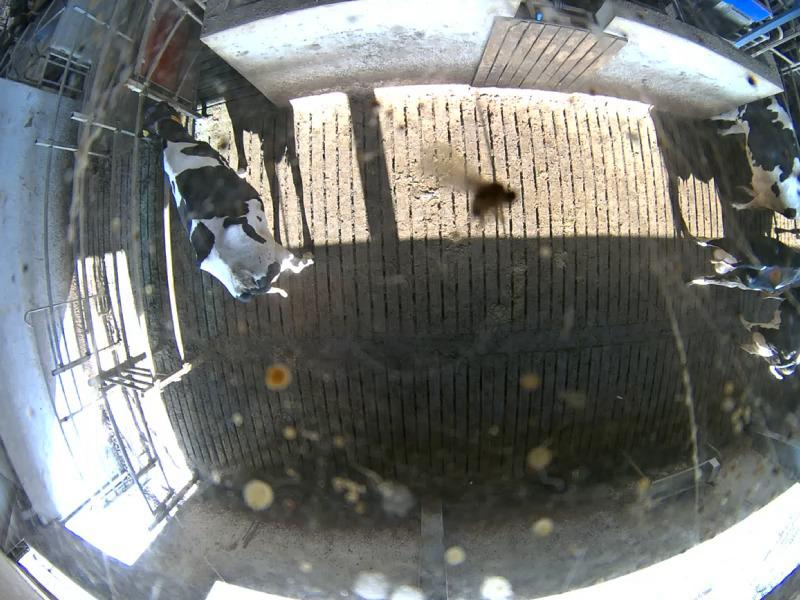
\includegraphics[width=0.3\textwidth]{new-2.jpg}
  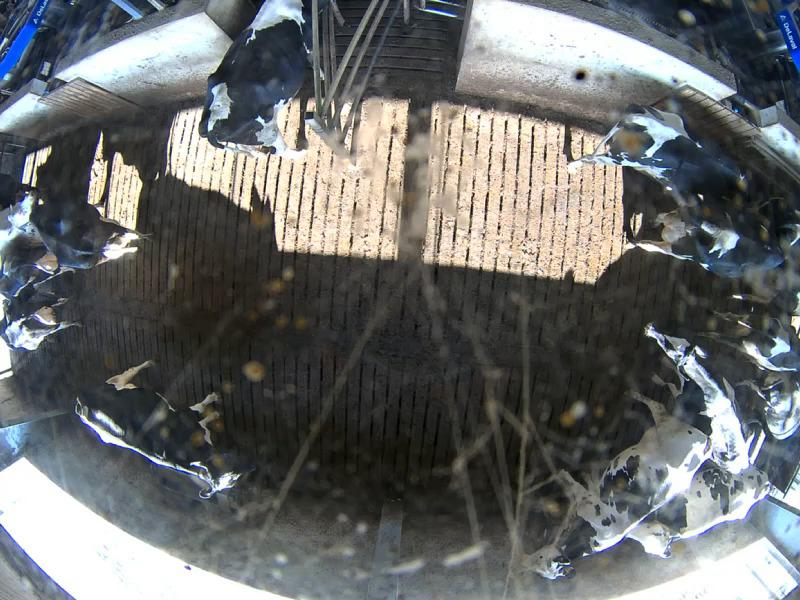
\includegraphics[width=0.3\textwidth]{new-1.jpg}
  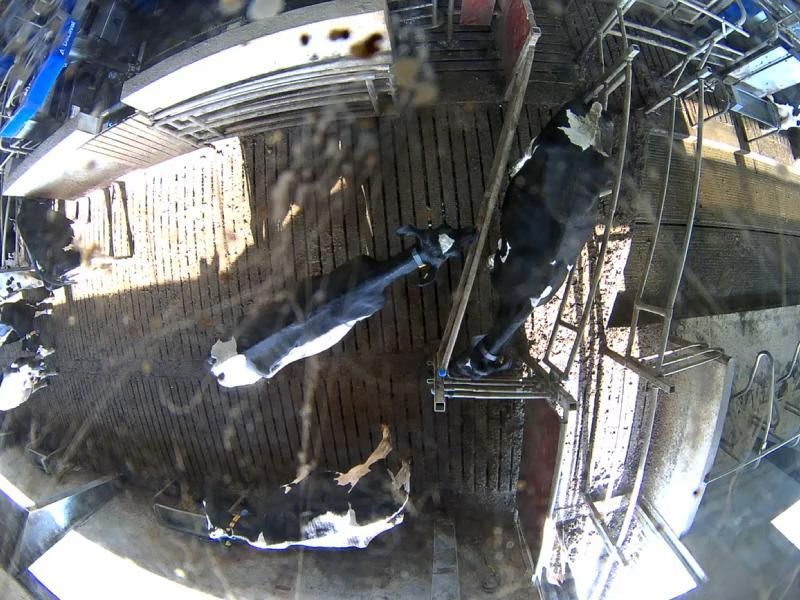
\includegraphics[width=0.3\textwidth]{new-0.jpg}
\end{center}
  \caption{Example frames from a second recording made half a year after the first one.}
  \label{fig:new}
\end{figure}

Half a year after the original recordings were made another month of video was collected, c.f Figure~\ref{fig:new}, and the original detector was tested on this data. It did however not perform very well. A set of 931 frames were sampled from the new recording and passed to the detector. It produced annotated images that were then inspected manually. Among these, 510 or 55\% of the images were perfectly interpreted in the same sense as above, while 421 or 45\% contained some sort of mistake.
A lot of false detections were made. Especially in over exposed areas and there were also more misses. 

Two main differences between this new data and the old one have been identified. 
First, the cameras have become quite dirty. They were cleaned a few times during the experiments, but they became dirty quite fast, so for a system like this to become useful it will have to be able to handle somewhat dirty cameras. Second, the sun was low in the sky during  the time of year of the new recording. That results in a different lighting situation. It is an indoor scene, but there are windows letting in the sun light.

From this new data, the 421 frames where the old detector made errors as well as 3 frames that contained no errors were manually annotated in the same way as before. They contained in total 2880 cows. The detector was retrained using both the new and the old data, which resulted in a detector with more even performance across the varying seasons. A validation set consisting of 10 \% of the annotated data (196 frames) was separated out and not used during the training. This set was used to evaluate the new detector. In total it contained 408 cows, and 396 of these were detected with only 6 extra detections. That gives an cow hit rate of 97 \% with a false alarm rate of 2.9 \%. In terms of frames 92.8 \% were perfectly interpreted while there were mistakes made in 14 of the frames. Among those 14, 13 contained more than one cow and thus the hit rate of the watchdog finding frames with two or more cows were 99.5 \%.

\subsection{Interaction detection}
To remove even more of the uninteresting video, an additional feature, the minimum distance between the cows in the scene, was also extracted. Then a short sequence containing a lot of interesting interactions consisting of 187 frames evenly sampled over 10 minutes was extracted and manually annotated by an expert. Five different interactions were identified: body pushing, butting, head butting, head pressing and body sniffing. Frames where any of these interactions were present, were considered interesting and all other frames uninteresting. The minimum cow distance, $d_f$, for each frame $f$, was extracted. It is believed to be a good feature as cows need to be close to interact. Also, the cows needs to be close for some period of time, so we take the maximum over 9 consecutive frames and use as feature, 
$x_f = \max_{f-4 \leq i < f+4} d_i$ for frame $f$.

By thresholding $x_f$ a simple detector is formed. By choosing different thresholds, the results could be varied between not detecting any uninteresting frames and not missing any interesting frames. Figure~\ref{fig:roc} shows the amount of the interesting frames detected (true positives) as a function of the amount of the uninteresting frames remaining (false positives) for different thresholds. It is, for example, possible to discard 20\% of the uninteresting frames while only losing 3\% of the interesting once. If it is acceptable to lose more of the interesting frames, even more of uninteresting frames could be discarded as detailed by the curve.

Note that this is in addition to the filtering by a number of cows performed in Section~\ref{sec:num}. By combining the two filters, 50\% of the uninteresting frames could be discarded while only loosing 4\% of the interesting frames.

\begin{figure}[tb]
\begin{center}
  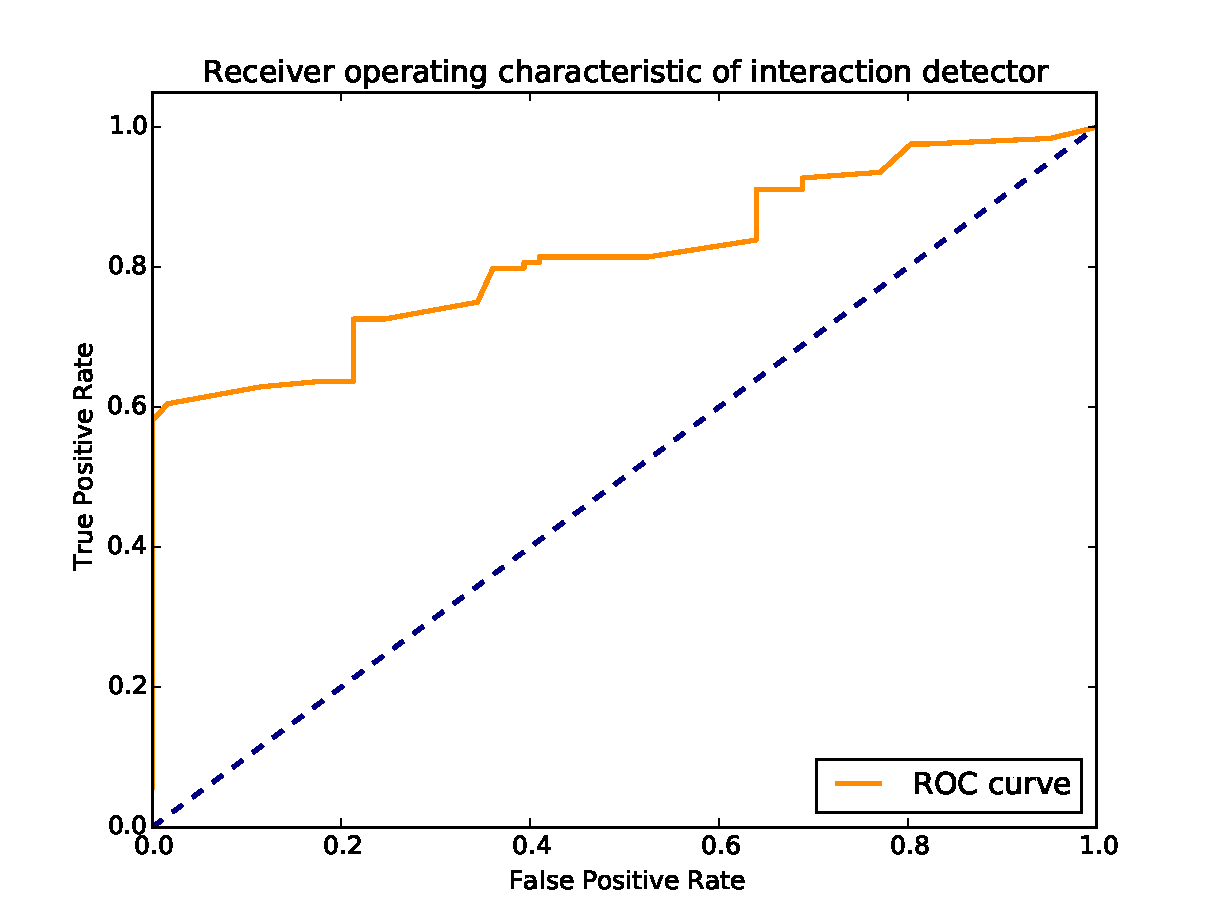
\includegraphics[width=0.75\textwidth]{roc.pdf}
\end{center}
  \caption{Results for different thresholds, with the amount of interesting frames kept (true positive rate) plotted as a function of the amount of uninteresting frames kept (false positive rate).}
  \label{fig:roc}
\end{figure}


\section{Conclusions}
A CNN cow detection system has been developed. It can detect and count the cows present in the image with high precision. 92.8 \% of the test images were perfectly interpreted in the sense that the system was able to place a rotated rectangle on each cow and nowhere else. This detector was used to discard 50 \% of the recorded video as uninteresting while only losing 4 \% of the interesting video. Regarding detection of single cows, the hitrate was 97 \% with a false alarm rate of 2.9 \%. 

Another important conclution was that the even though it is an indoor scene, the lighting variations caused by the varying seasons are significant. It was not enought to collect data from a single month. Insted both traning data and evalutation data from different seasons are needed to build a system that can operate all year around. This seems to concur with the findings of Porto et al. \cite{porto2015automatic} who write that their detector, CVBS 
"were highly affected by the shadows" and that "worst operating
conditions for the CVBS occurred in the summer".


\section{Acknowledgement}
The computations were performed on resources provided by the Swedish National Infrastructure for Computing (SNIC) at Lunarc. The Swedish Research Council for Environment, Agricultural Sciences and 
Spatial Planning (FORMAS) is acknowledged 
for the funding of the project. The farmer, Mikael Palm, is acknowledged for the use of his diary bran and cows during the pilot studie.



\bibliographystyle{plain}
{\parindent0pt
\parskip8pt
\bibliography{main}
}
\end{document}
